\section*{Scenario 2: Disaster Preparedness — Identifying Flood-Prone Regions}

Flood preparedness is a crucial step in climate resilience, particularly in regions where seasonal rainfall patterns lead to recurring floods. By analyzing historical rainfall data, we can identify areas most at risk and proactively design early warning systems, resource allocation strategies, and infrastructure improvements.

\subsection*{Objective}
\begin{itemize}
    \item Identify the top 5 regions with the highest average rainfall.
    \item Recommend the months in which flood alerts should be heightened based on high monthly rainfall.
\end{itemize}

\subsection*{R Code for Analysis}
\textbf{Top 5 Rainfall-Prone Regions:}
\begin{verbatim}
# Aggregate rainfall by region
region_rainfall <- climate_data %>%
  group_by(District) %>%
  summarise(avg_rainfall = mean(Precip, na.rm = TRUE)) %>%
  arrange(desc(avg_rainfall))

# Show the top 5 regions with highest rainfall
top_regions <- head(region_rainfall, 5)
print(top_regions)
\end{verbatim}

\begin{table}[h!]
\centering
\begin{tabular}{|c|c|}
\hline
\textbf{District} & \textbf{Average Rainfall (mm)} \\
\hline
Ilam & 3.64 \\
Jhapa & 3.39 \\
Argakhanchi & 3.03 \\
Rupandehi & 3.03 \\
Palpa & 3.02 \\
\hline
\end{tabular}
\caption{Top 5 Rainfall-Prone Districts}
\end{table}

\subsection*{Monthly Rainfall in Top Regions}

To identify critical months for potential flood risks, we examined the monthly average rainfall in each of the top-ranking districts. This analysis highlights temporal patterns of precipitation, allowing for a clearer understanding of seasonal variability. Months with the highest recorded precipitation in each district should be prioritized in flood alert planning and early warning systems.


\textbf{R Code:}
\begin{verbatim}
monthly_rainfall <- climate_data %>%
  filter(District %in% top_regions$District) %>%
  group_by(District, Month) %>%
  summarize(Monthly_Rainfall = mean(Precip, na.rm = TRUE)) %>%
  arrange(District, desc(Monthly_Rainfall))

ggplot(monthly_rainfall, aes(
  x = District, y = Monthly_Rainfall, fill = Month)) +
  geom_bar(stat = "identity", position = "dodge") +
  scale_fill_brewer(palette = "Set3") +
  labs(
    title = "Monthly Rainfall Distribution in Top Regions",
    x = "District",
    y = "Average Monthly Rainfall (mm)",
    fill = "Month"
  ) +
  theme_minimal() +
  theme(
    axis.text.x = element_text(angle = 45, hjust = 1),
    legend.position = "right"
  )
\end{verbatim}

% Figure here-----------------------------
\begin{figure}[h]
\centering
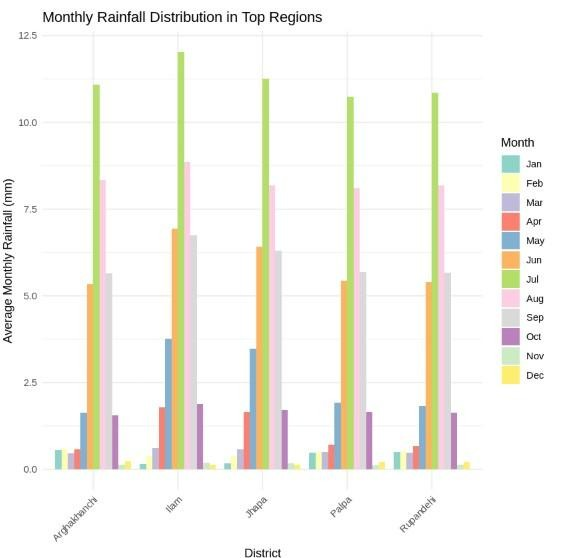
\includegraphics[width=0.5\textwidth]{figures/case2.jpg}
\caption{Figure 8.2: Monthly Rainfall Distribution in Top Rainfall-Prone Districts}
\end{figure}

\subsection*{Conclusion}

This analysis pinpoints both vulnerable districts and high-risk months. Such data-backed insights empower regional authorities to:
\begin{itemize}
    \item Issue timely flood warnings.
    \item Allocate emergency resources.
    \item Plan preventive infrastructure improvements.
\end{itemize}
